Este gráfico se basa en el principio de Pareto. Realizar un diagrama de Pareto ayuda a identificar estas "pocas causas" que, al resolverlas, se resuelven buena parte de los problemas.

    \resumebox{definicion}{Principio de Paretto}{Unas pocas causas son las que crean los mayores efectos.}

La realización de un diagrama de Paretto parte por la determinación de la situación general. Una vez conocido el problema general se determinan en qué categorías se catalogarán los problemas del proceso. Con esto listo se puede iniciar la recolección de datos alrededor de los problemas de un proceso y la asignación de cada uno de estos en una de las categorías determinadas.

Una vez se tienen los datos recolectados, lo primero a realizar es ordenarlos de mayor a menor. Posterior a esto, se calcula el porcentaje ($\%$, \autoref{eq:pareto_porcentaje}) que cada categoría representa de la cantidad de problemas total, así como el porcentaje acumulado ($\%_{Ac}$, \autoref{eq:pareto_porcentaje_acumulado}) de las categorías

\begin{equation}\label{eq:pareto_porcentaje}
    \% = 100\cdot\frac{x_{i}}{\sum{x_{i}}}
\end{equation}

\begin{equation}\label{eq:pareto_porcentaje_acumulado}
    \%_{Ac} = \sum{\%}
\end{equation}

Una vez se tienen todos estos datos, se elabora una gráfica con los datos ordenados de la siguiente manera

\begin{itemize}
    \item Eje X: Categorías de problemas
    \item Eje Y (Izquierda): Conteo de observaciones
    \item Eje Y (Derecha): Porcentaje acumulado
\end{itemize}

Con la gráfica lista, procedemos a trazar una linea en el punto en que se cruza el 80\% de porcentaje acumulado.

\begin{figure}\centering
    \resizebox{\linewidth}{!}{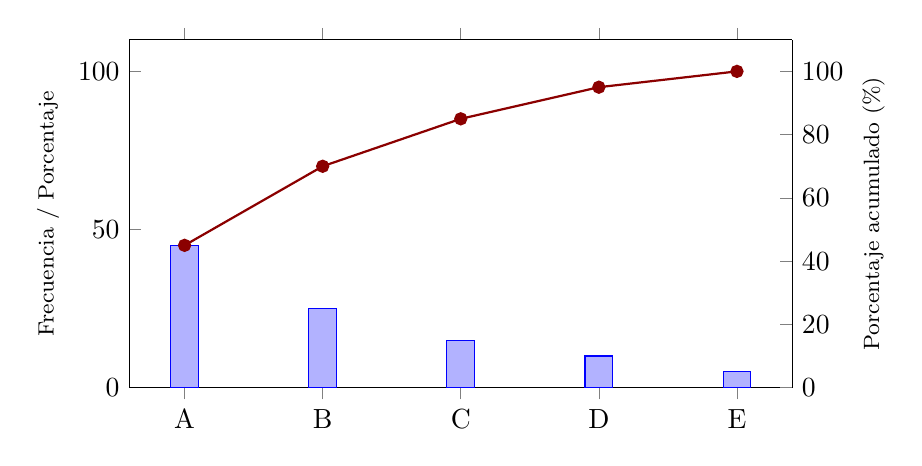
\begin{tikzpicture}
  \begin{axis}[
      width=10cm,height=6cm,
      ybar,ymin=0,ymax=110,
      axis y line*=left,
      ylabel={\footnotesize Frecuencia / Porcentaje},
      symbolic x coords={A, B, C, D, E},
      xtick=data
    ]
    \addplot coordinates {(A,45) (B,25) (C,15) (D,10) (E,5)};
  \end{axis}

  \begin{axis}[
      width=10cm,height=6cm,
      ymin=0,ymax=110,
      axis y line*=right,
      ytick={0,20,40,60,80,100},
      ylabel={\footnotesize Porcentaje acumulado (\%)},
      axis x line=none,
      symbolic x coords={A, B, C, D, E},
      xtick=data
    ]
    \addplot[DarkRed, thick, mark=*] coordinates {(A,45) (B,70) (C,85) (D,95) (E,100)};
  \end{axis}
\end{tikzpicture}}
    \rule{\linewidth}{0.5pt}
    \caption{Ejemplo de diagrama de Paretto}
    \label{fig:diagrama_de_pareto}
\end{figure}